\subsection{Classifier Performance}
\label{sec:constraintdetection}

Our first experiment evaluates how model and prompt design affect the accuracy of constraint classification. Starting from the prompt in Figure~\ref{fig:classifyprompt} (Section~\ref{sec:classifier}), we derive four
variants by enabling or disabling \emph{constraint examples} and
\emph{table context}: \emph{No Context}, \emph{Table Context},
\emph{Examples}, and \emph{Examples + Table Context}. We evaluate all four variants across six LLMs and all \DIFdelbegin \DIFdel{four }\DIFdelend \DIFaddbegin \DIFadd{six }\DIFaddend datasets. Figure~\ref{fig:classifier-results} summarizes the results. Because sentences missed at this stage cannot be recovered later by the mapper, we require a recall of at least 0.90 \DIFaddbegin \DIFadd{on every dataset }\DIFaddend when selecting a default configuration (red dashed line).

\begin{figure}[!ht]
    \centering
    \DIFdelbeginFL %DIFDELCMD < 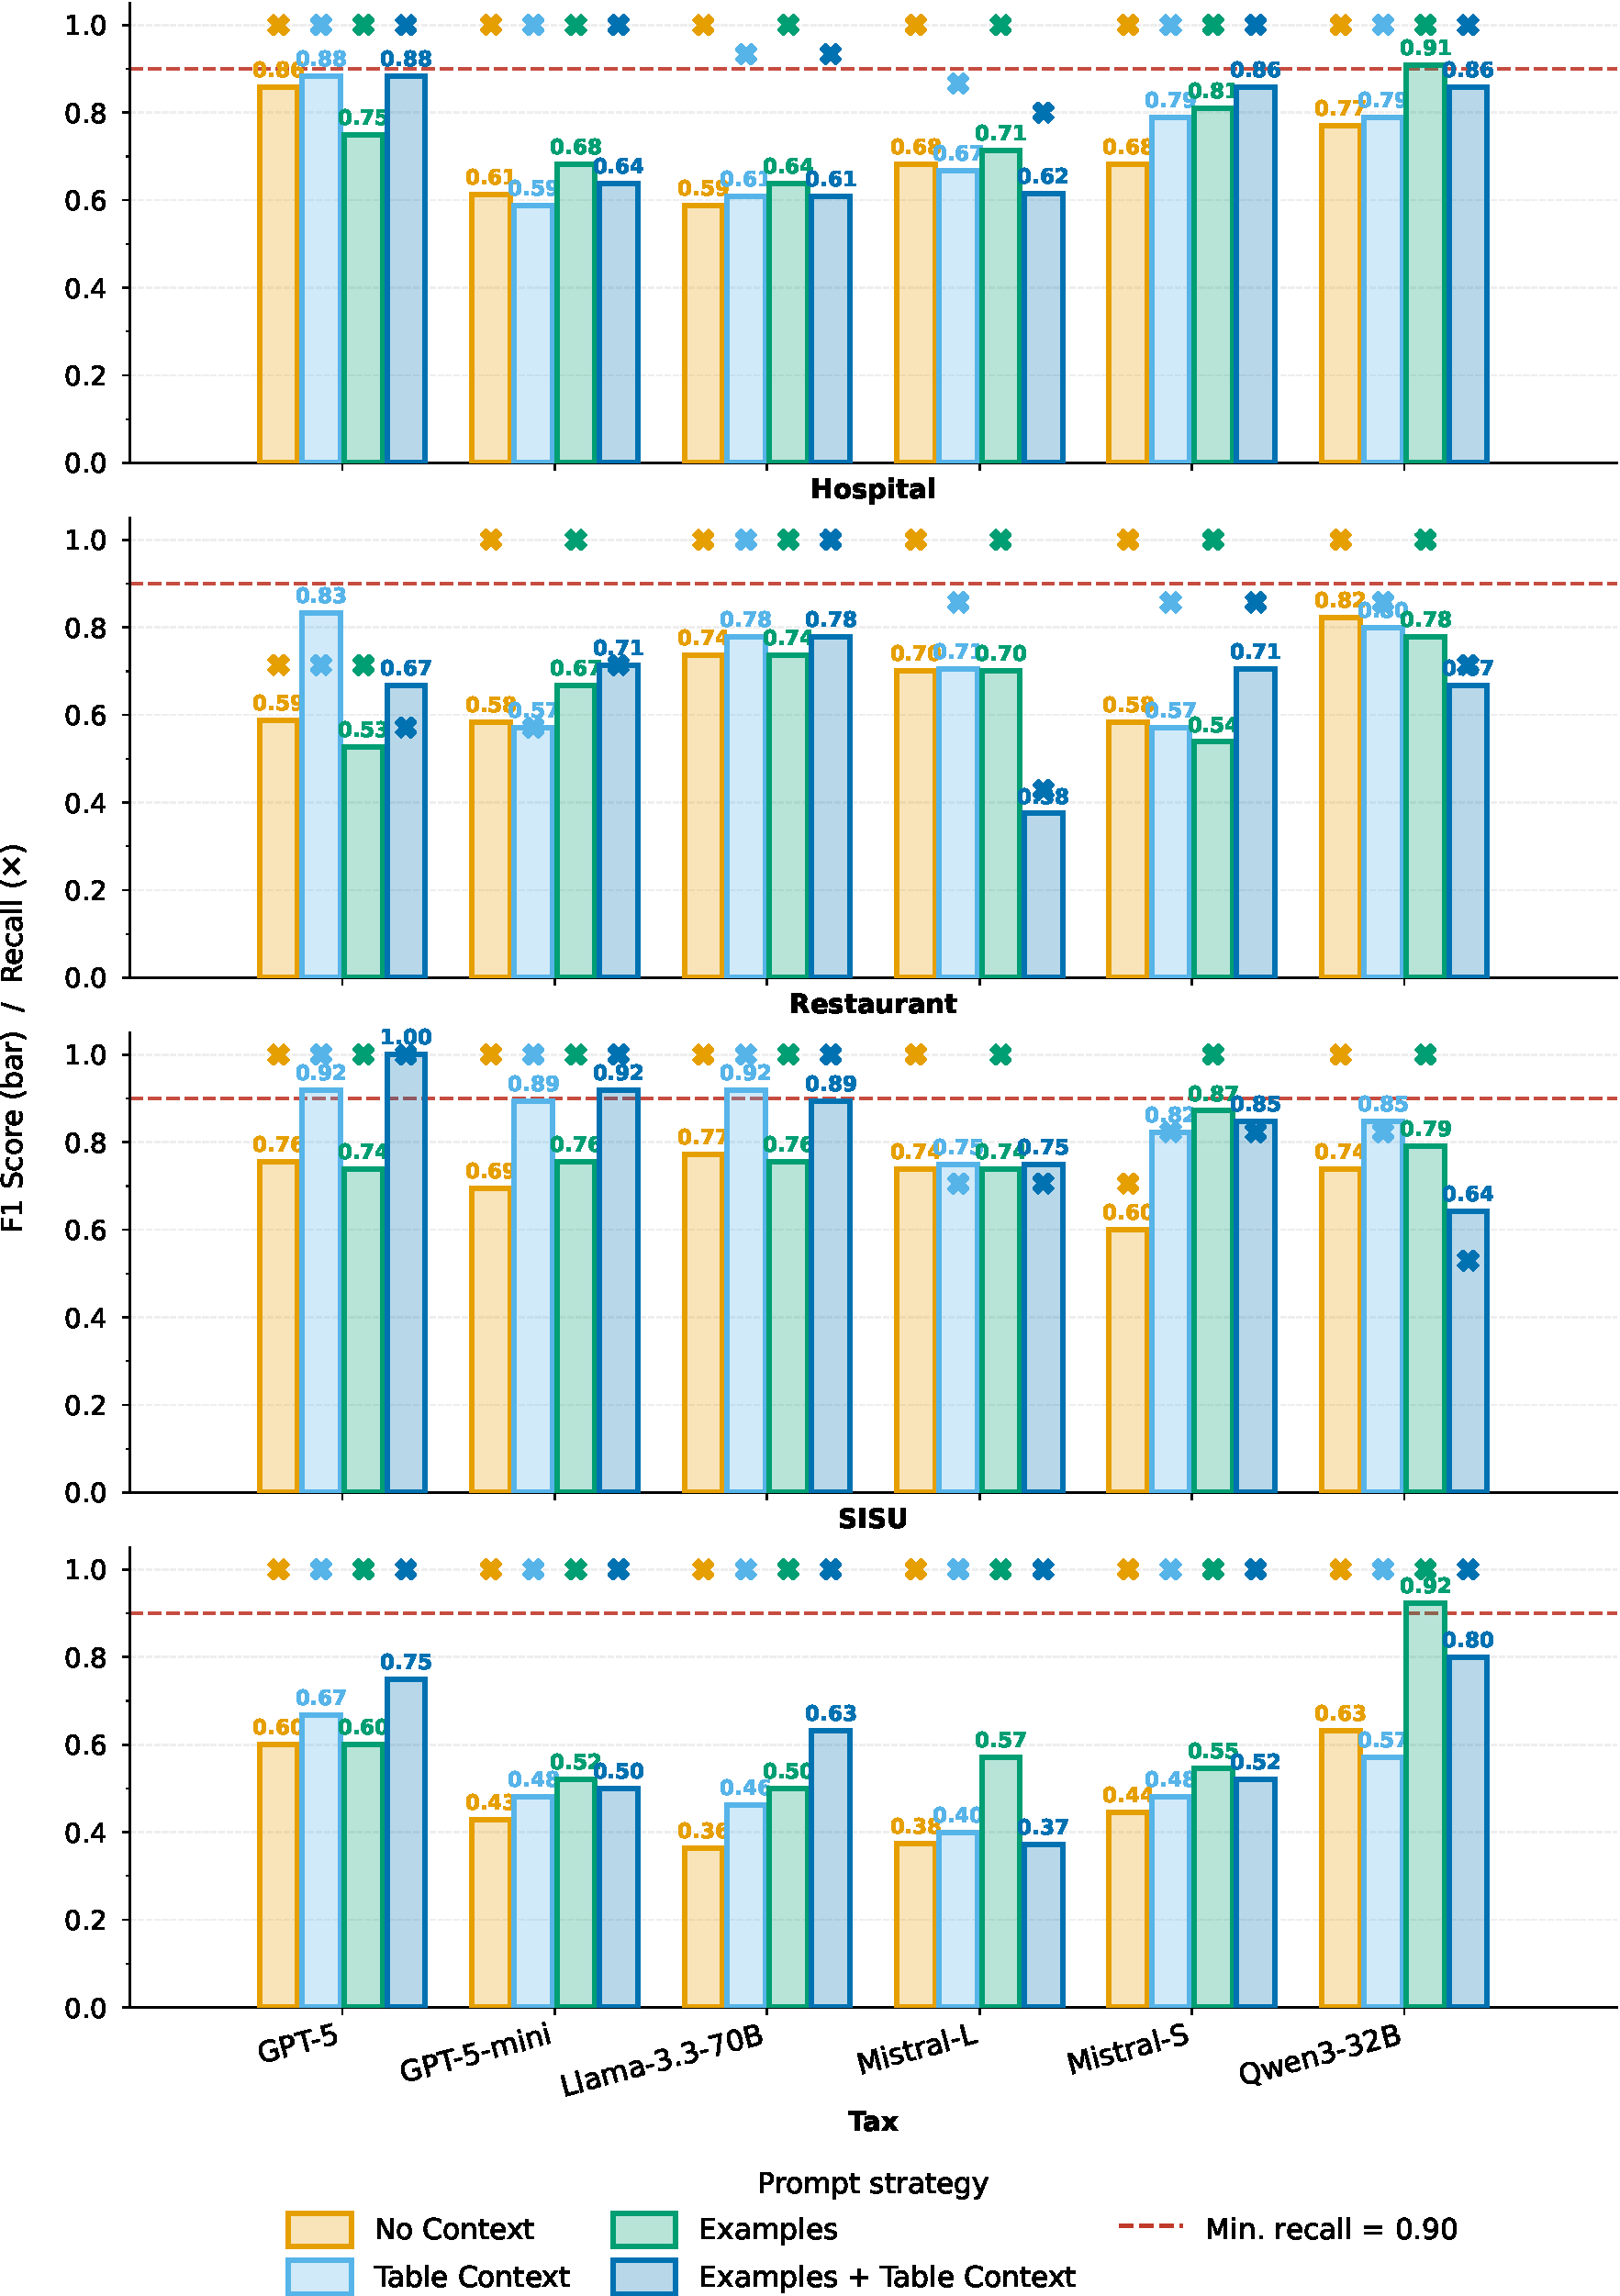
\includegraphics[width=\columnwidth]{figures/results/classifier_ablation.pdf}
%DIFDELCMD < %%%
\DIFdelendFL \DIFaddbeginFL 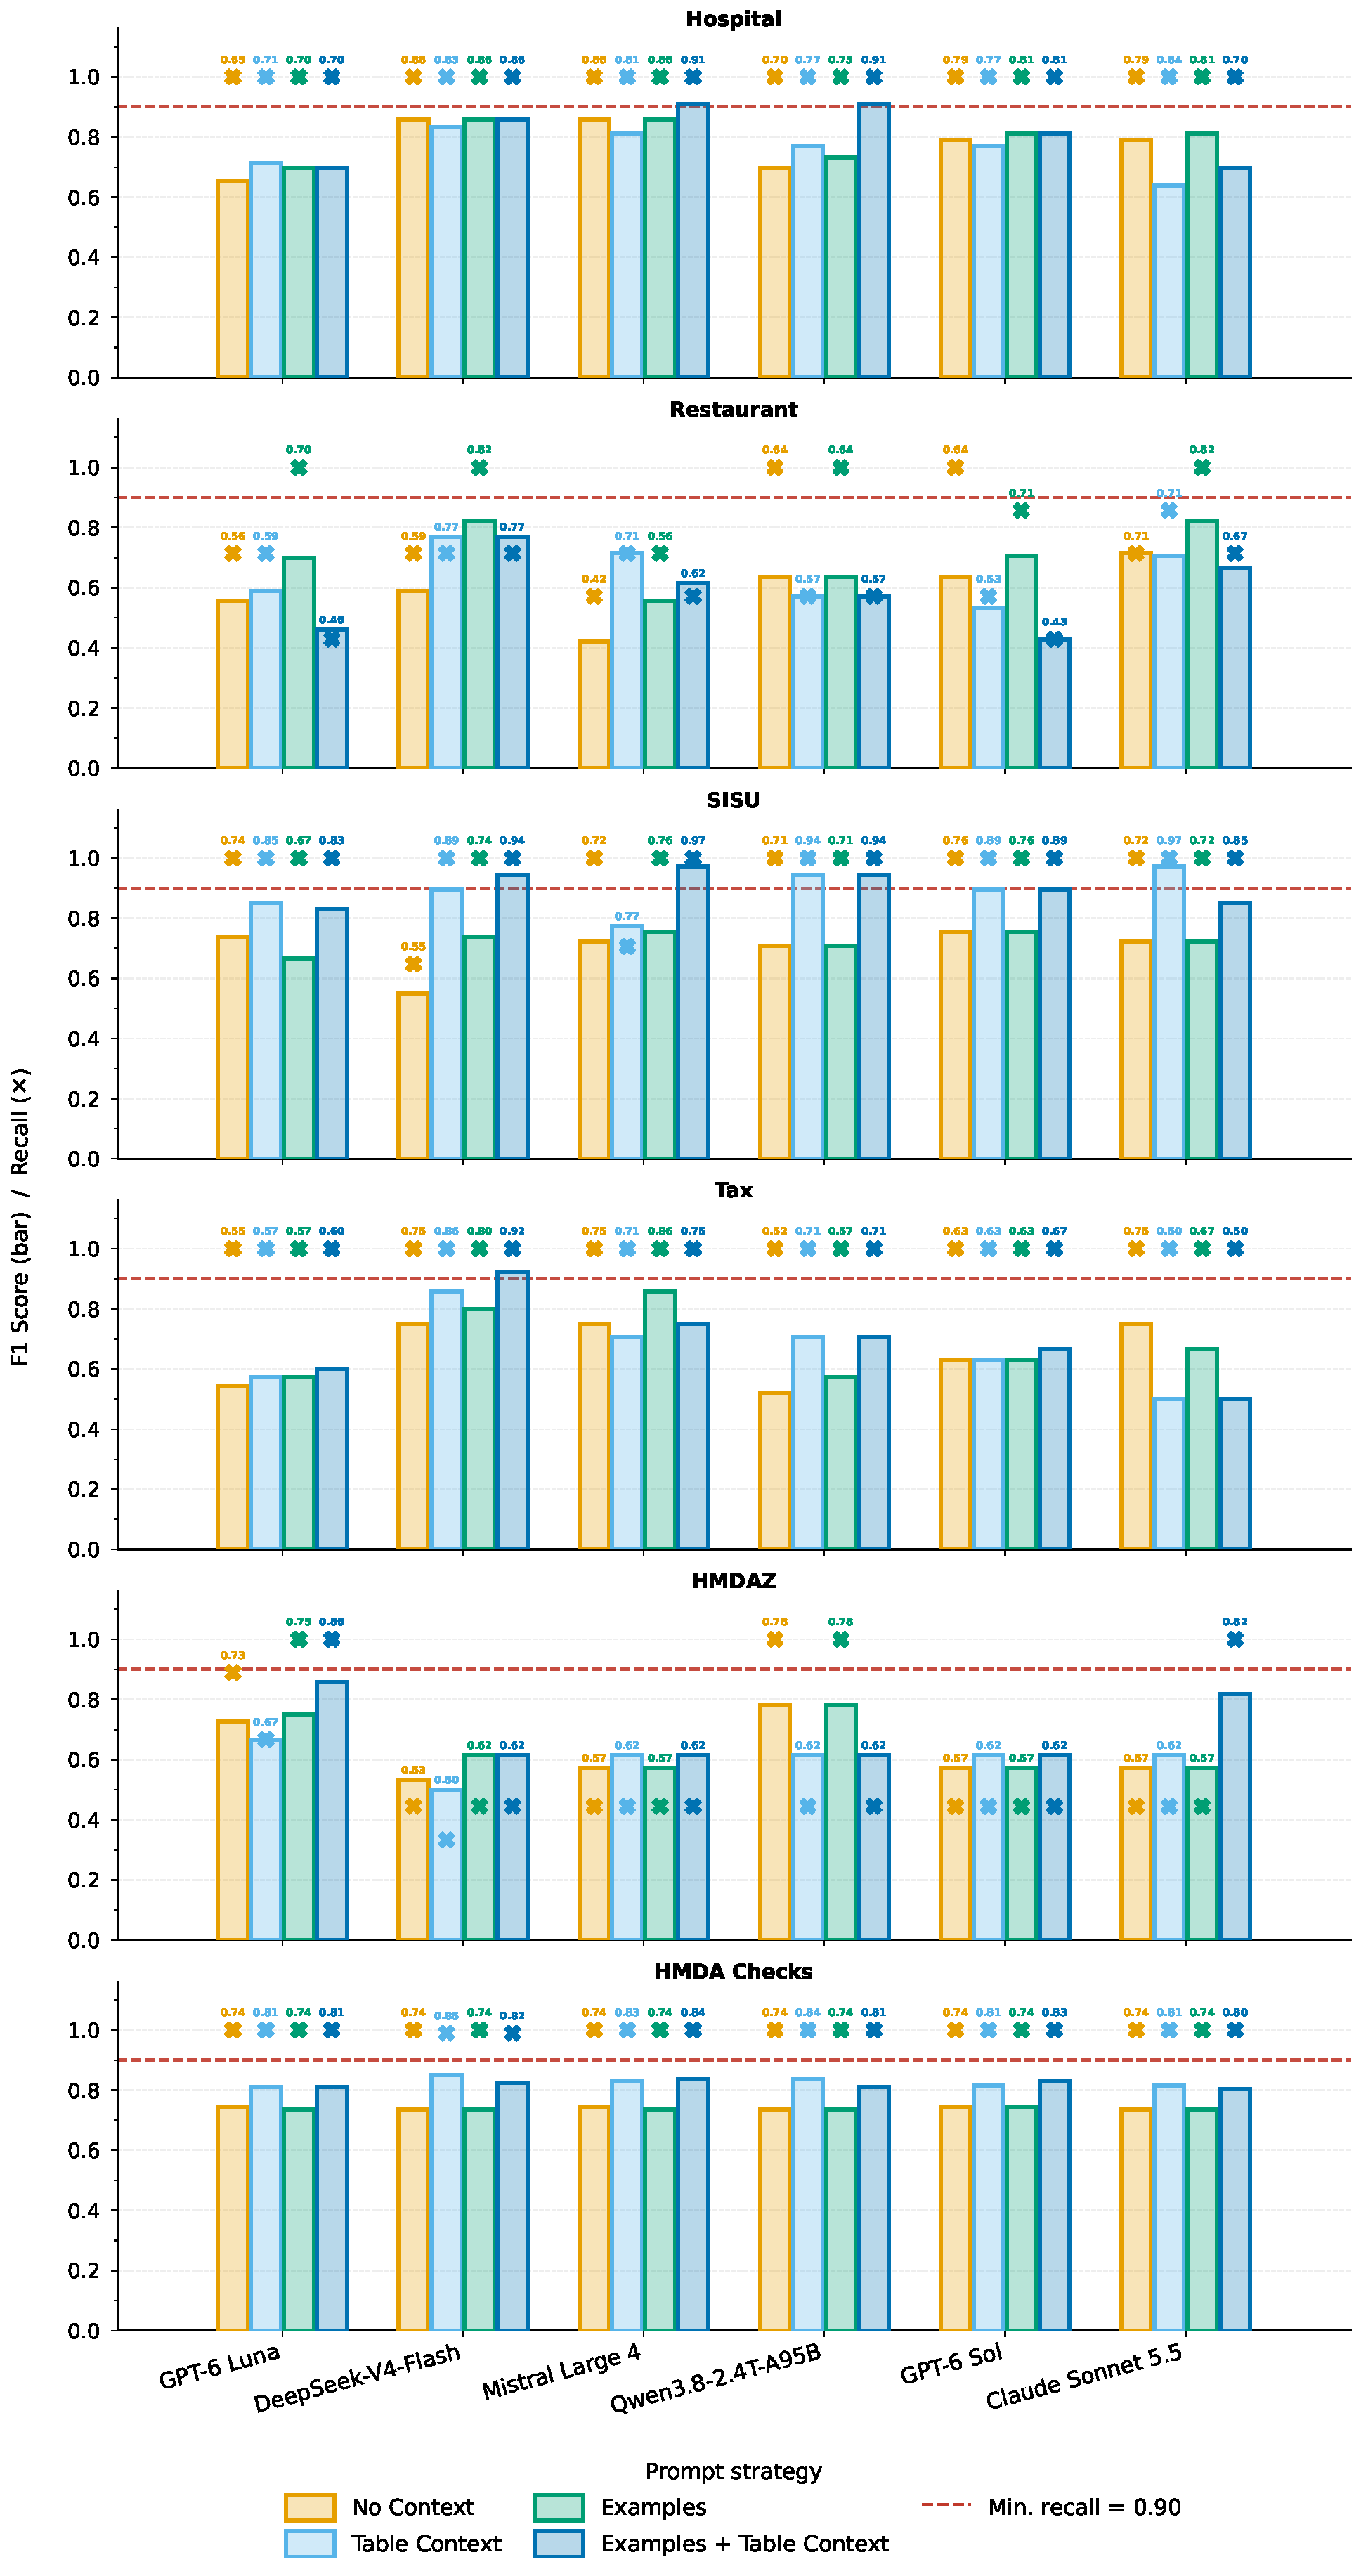
\includegraphics[width=\columnwidth]{figures/results/v3_fig6_classifiers.pdf}
\DIFaddendFL \caption{Constraint classification F$_1$ (bars) and recall (\textsf{x}) across models and prompt variants. The dashed line marks the 0.90 recall threshold.}
    \label{fig:classifier-results}
\end{figure}

\DIFdelbegin \DIFdel{Most configurations achieve recall
close to or equal to }\DIFdelend \DIFaddbegin \DIFadd{On Hospital, Tax, SISU, and HMDA Checks, almost every configuration reaches recall
}\DIFaddend 1.00, \DIFdelbegin \DIFdel{indicating that constraint classification is a reliable first stage for }%DIFDELCMD < \system%%%
\DIFdel{. The main differences appear in precisionand}\DIFdelend \DIFaddbegin \DIFadd{so the differences lie in precision. HMDAZ and Restaurant behave
differently: there, recall is the bottleneck. On HMDAZ, most configurations
recover only 4 of the 9 constraint sentences (recall 0.44). The missed sentences
are regulatory definitions (e.g.}\DIFaddend , \DIFdelbegin \DIFdel{consequently, in F$_1$. A key observation is that a task definition alone is not sufficient. Without
examples or table context, models produce more false positives, especially on sentences that mention the domain but do not state a data constraint . Adding examples or table context often improves precision.Examples provide concrete positive and negative cases for calibration, while the table context helps the model assess whether a sentence can be linked to the available columns.}%DIFDELCMD < 

%DIFDELCMD < %%%
\DIFdel{Overall, }\emph{\DIFdel{Examples}} %DIFAUXCMD
\DIFdel{is the most robust option across models and datasets. Among the configurations that meet }\DIFdelend \DIFaddbegin \DIFadd{when a mortgage is high-cost) that read as
scope statements, although each implies a checkable condition on the data. Only three configurations satisfy }\DIFaddend the recall requirement \DIFdelbegin \DIFdel{across all datasets, the top-performing ones consistently include examples. }\DIFdelend \DIFaddbegin \DIFadd{on all six datasets:
}\emph{\DIFadd{Qwen3.8-2.4T-A95B}} \DIFadd{with }\emph{\DIFadd{Examples}} \DIFadd{(mean F$_1$ 0.69),
}\DIFaddend \emph{\DIFdelbegin \DIFdel{Qwen3-32B}\DIFdelend \DIFaddbegin \DIFadd{GPT-6 Luna}\DIFaddend } with \emph{Examples} \DIFdelbegin \DIFdel{performs best overall, }\DIFdelend \DIFaddbegin \DIFadd{(0.69), and }\emph{\DIFadd{Qwen3.8-2.4T-A95B}} \DIFadd{with
}\emph{\DIFadd{No Context}} \DIFadd{(0.68). As in our previous evaluation, the qualifying configurations
are dominated by }\emph{\DIFadd{Examples}}\DIFadd{, and we select }\emph{\DIFadd{Qwen3.8-2.4T-A95B}} \DIFaddend with
\DIFdelbegin \DIFdel{a }\DIFdelend \DIFaddbegin \emph{\DIFadd{Examples}} \DIFadd{as the default classifier. Configurations with higher }\DIFaddend mean F$_1$
\DIFdelbegin \DIFdel{of }\DIFdelend \DIFaddbegin \DIFadd{exist (e.g., DeepSeek-V4-Flash with }\emph{\DIFadd{Examples + Table Context}}\DIFadd{, 0.82), but
they miss more than half of the HMDAZ constraints.
}

\DIFadd{Table context has two opposite effects. It is the only signal that raises
precision on HMDA Checks: without it, the models label (almost) every edit as a
constraint, and F$_1$ equals that of the trivial all-positive classifier (0.74).
The non-constraint edits are phrased exactly like the checkable ones and differ
only in that they refer to aggregates, the transmittal sheet, or external
reference data; we conjecture that the record layout shown in the table context
is what lets the model tell them apart. With table context, F$_1$ rises
to 0.80--0.85. On wide schemas, however, the same context does not
help recall: on HMDAZ (135 columns), 9 of the 12 table-context configurations
stay at or below 0.44, and only GPT-6 Luna and Claude Sonnet 5.5 with
}\emph{\DIFadd{Examples + Table Context}} \DIFadd{recover all nine constraint sentences. Averaged over all models and datasets, }\emph{\DIFadd{Examples}} \DIFadd{gives the best recall (0.93), while the table-context variants give higher precision (0.71 vs.\ 0.58--0.62) at the cost of recall (}\DIFaddend 0.85\DIFdelbegin \DIFdel{across datasets.
Adding table context on top of examples yields mixed results: while itcan improve performance in some cases, it can also degrade it, possibly due to increased prompt length and noise introduced by schema details and sample tuples. We therefore select }\emph{\DIFdel{Qwen3-32B}} %DIFAUXCMD
\DIFdel{with
}\DIFdelend \DIFaddbegin \DIFadd{--0.87).
}

\DIFadd{Compared with the backbones of our previous evaluation, the current models are,
on average, better classifiers on the four original datasets (mean F$_1$ 0.72
vs.\ 0.69 across all configurations), but the best configuration that satisfies
the recall constraint is weaker (0.66 on those four datasets vs.\ 0.85 for
Qwen3-32B with }\DIFaddend \emph{Examples}\DIFdelbegin \DIFdel{as the default classifier for the remaining experiments.
}\DIFdelend \DIFaddbegin \DIFadd{). Newer models tend to accept more sentences as
constraints, which keeps recall high but lowers precision, especially on Tax and
Restaurant.
}\DIFaddend \altic{[R3-O4] Analisar POR QUE o classificador já vai bem sem contexto/exemplos (ganhos marginais, sobretudo no GPT). Discutir a hipótese do revisor: possível exposição a esses datasets/texto regulatório no pré-treino. Mitigar/avaliar: comparar datasets sintéticos vs. SISU/Restaurant, e relacionar com a discussão de vazamento de priors em [R2-O6.2].}
 \DIFdelbegin %DIFDELCMD < 

%DIFDELCMD < %%%
\DIFdel{This result aligns with our use of few-shot prompting, where generic task-level examples help guide the model’s decision-making even in the absence of domain-specific supervision.}%DIFDELCMD < 

%DIFDELCMD <  %%%
\DIFdelend